% generated by tools/v10/fe_crops.py: insets of the Frame Explorer captures, cut from the lossless 1280x720 captures (pixels not resampled)
\newcommand{\feStageVertexFormula}{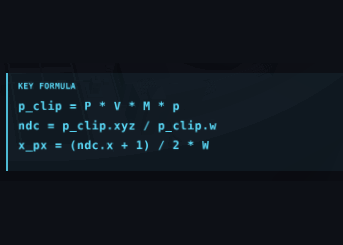
\includegraphics[width=80.15mm]{figures/img/fecrops/feStageVertexFormula.png}}
\newcommand{\feStageVertexInfo}{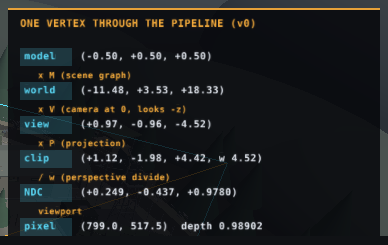
\includegraphics[width=90.67mm]{figures/img/fecrops/feStageVertexInfo.png}}
\newcommand{\feStageAssemblyFormula}{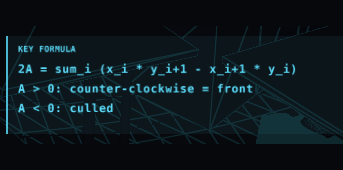
\includegraphics[width=80.15mm]{figures/img/fecrops/feStageAssemblyFormula.png}}
\newcommand{\feStageAssemblyInfo}{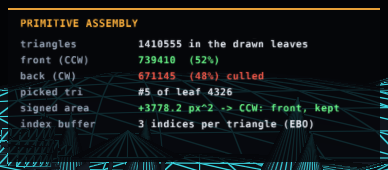
\includegraphics[width=90.67mm]{figures/img/fecrops/feStageAssemblyInfo.png}}
\newcommand{\feStageDepthFormula}{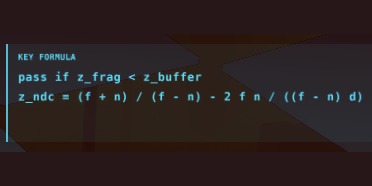
\includegraphics[width=83.7mm]{figures/img/fecrops/feStageDepthFormula.png}}
\newcommand{\feStageDepthInfo}{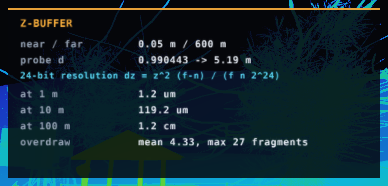
\includegraphics[width=87.3mm]{figures/img/fecrops/feStageDepthInfo.png}}
\newcommand{\feRasterScanFormula}{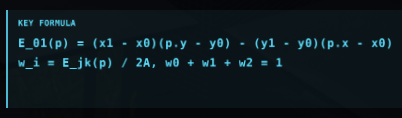
\includegraphics[width=93.9mm]{figures/img/fecrops/feRasterScanFormula.png}}
\newcommand{\feRasterScanInfo}{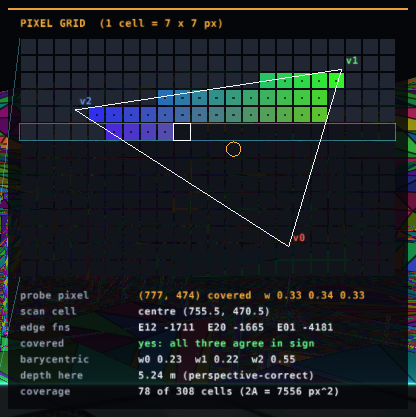
\includegraphics[width=97.2mm]{figures/img/fecrops/feRasterScanInfo.png}}
\newcommand{\feInterpAffinePerspectiveFormula}{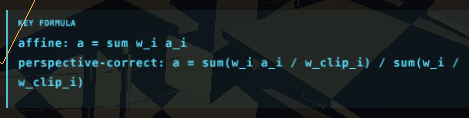
\includegraphics[width=109.6mm]{figures/img/fecrops/feInterpAffinePerspectiveFormula.png}}
\newcommand{\feInterpAffinePerspectiveInfo}{\raisebox{0pt}[\dimexpr\height+2mm\relax][0pt]{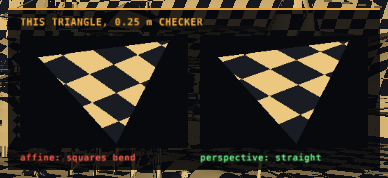
\includegraphics[width=97.2mm]{figures/img/fecrops/feInterpAffinePerspectiveInfo.png}}}
\newcommand{\feInterpGouraudPhongFormula}{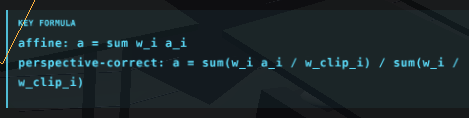
\includegraphics[width=109.6mm]{figures/img/fecrops/feInterpGouraudPhongFormula.png}}
\newcommand{\feInterpGouraudPhongInfo}{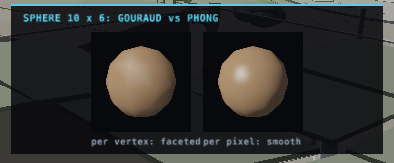
\includegraphics[width=92.1mm]{figures/img/fecrops/feInterpGouraudPhongInfo.png}}
\newcommand{\feStageTaaFormula}{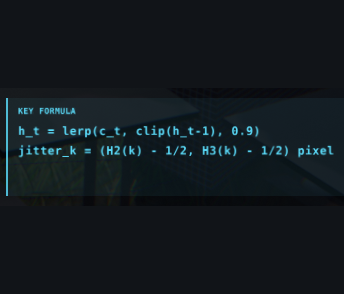
\includegraphics[width=80.36mm]{figures/img/fecrops/feStageTaaFormula.png}}
\newcommand{\feStageTaaInfo}{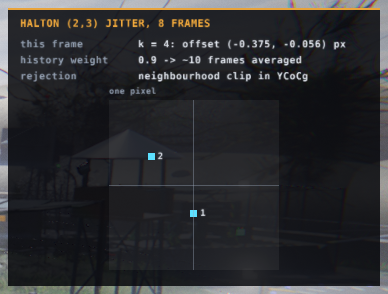
\includegraphics[width=90.63mm]{figures/img/fecrops/feStageTaaInfo.png}}
\newcommand{\feImagelabGaussGammaKernel}{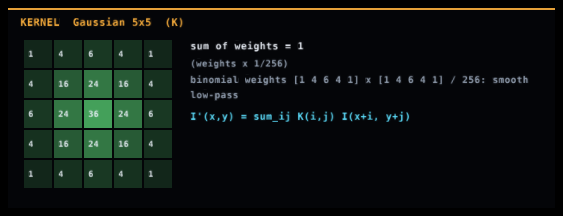
\includegraphics[width=131.6mm]{figures/img/fecrops/feImagelabGaussGammaKernel.png}}
\newcommand{\feImagelabSobelKernel}{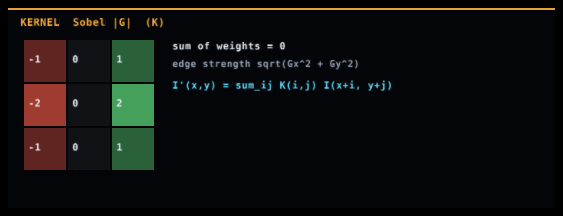
\includegraphics[width=131.6mm]{figures/img/fecrops/feImagelabSobelKernel.png}}
